\documentclass[11pt,letterpaper]{article}
\usepackage{fullpage}
\usepackage{multicol}
\usepackage{amsmath}
\usepackage{amsfonts}
\usepackage{amssymb}
\usepackage{graphicx}
%\usepackage{pstricks, pst-node, pst-plot}

\newcommand{\ds}{\displaystyle}
\newcommand{\bv}{\mathbf}
\newcommand{\lv}{\langle}
\newcommand{\rv}{\rangle}

\begin{document}
\flushleft
\begin{multicols}{2}


\begin{large}\textbf{Math 115 Extra Credits \\ \hfill Fall 2010     }\end{large}

\vspace{.5in}

\end{multicols}

\pagestyle{empty}

\flushleft

Points from extra credit go to your total quiz score.

\begin{description}
 \item[Week 3 (2 pts)] p. 59 \# 34
\begin{enumerate}
\renewcommand{\labelenumi}{(\alph{enumi})}
 \item Here, $f(x)=\frac{e^x-1}{x}$.

\vspace{.5pc}
\begin{tabular}{rl}
$x$ & $f(x)$ (to 5 decimal places) \\
-0.1 & 0.95163 \\
-0.01 & 0.99502 \\
-0.001 & 0.99950 \\
-0.0001 & 1.00000 \\
0.0001 & 1.00010 \\
0.001 & 1.00050\\
0.01 & 1.00502 \\
0.1 & 1.05170 \\
 \end{tabular}

\item Conjecture: $\lim_{x\rightarrow 0}f(x)=1.00005$, which is between $f(-0.0001)$ and $f(0.0001)$.

\item The function is defined everywhere except at $x=0$.

\vspace{.1pc}
\begin{center}
 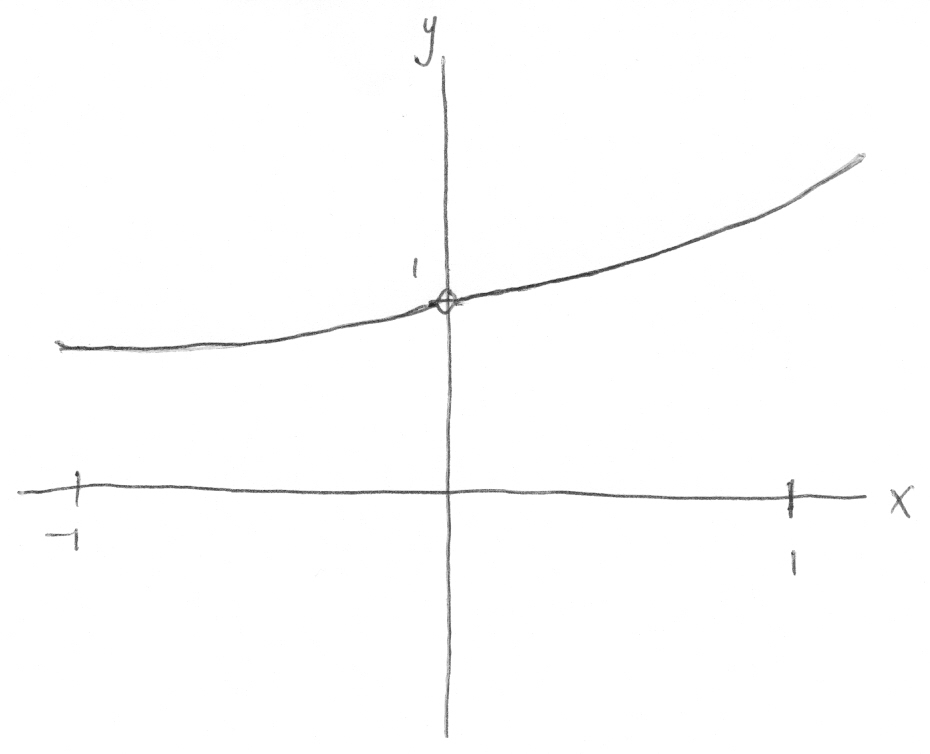
\includegraphics[scale=.4]{ecpic0001.jpg}
\end{center}

\item From the table in (a), $x\in \left[-0.01,0.01\right]$ is a suitable interval.

\end{enumerate}

 \item[13 Oct (1 pt)]
Differentiate the following with respect to $x$.
\begin{enumerate}
 \item $y=6$; $y'=0$
\item $y=5x$; $y'=5$
\item $y=21x^3+9x$; $y'=63x^2+9$
\item $y=x^2+2x-1$; $y'=2x+2$
\item $y=a_nx^n+a_{n-1}x^{n-1}+\dots a_1x+a_0$; $y'=na_nx^{n-1}+(n-1)a_{n-1}x^{n-2}+\dots +a_1$
\end{enumerate}

\item[27 Oct (1 pt)] Use the quotient rule to find
\[\frac{d}{dx}\left(\tan{x}=\frac{\sin{x}}{\cos{x}}\right).\]
\begin{eqnarray*}
 \frac{d}{dx}\tan{x} &=& \frac{\cos{x}\cos{x}-\sin{x}(-\sin{x})}{\cos^2{x}} \\
&=& \frac{\cos^2{x}+\sin^2{x}}{\cos^2{x}} \\
&=& \frac{1}{\cos^2{x}} \\
&=& \sec^2{x}.
\end{eqnarray*}

\item[1 Nov (1 pt)]  Compute $\frac{d}{dx}\arcsin{x}$ using the right triangle.

\vspace{.5pc}
Since $\sin{(\arcsin{x})}=x$, implicit differentiation gives
\begin{eqnarray*}
 1 &=& \frac{d}{dx}\sin{(\arcsin{x})} \\
&=& \cos{(\arcsin{x})}\cdot \frac{d}{dx}\arcsin{x} \\
\frac{1}{\cos{(\arcsin{x})}} &=& \frac{d}{dx}\arcsin{x}. 
\end{eqnarray*}
\begin{center}
 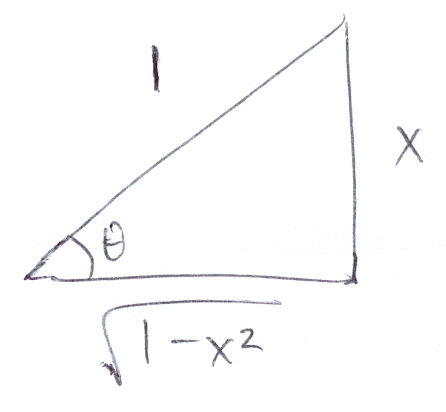
\includegraphics[scale=.2]{ecpic20001.jpg}
\end{center}
In the right triangle, $\sin{\theta }=x$ so $\arcsin{x}=\theta $.  Then
\begin{eqnarray*}
 \frac{d}{dx}\arcsin{x} &=& \frac{1}{\cos{(\arcsin{x})}} \\
&=& \frac{1}{\cos{\theta }} \\
&=& \frac{1}{\frac{\sqrt{1-x^2}}{1}} \\
&=& \frac{1}{\sqrt{1-x^2}}.
\end{eqnarray*}

\item[2 Dec (1 pt)]  Using $\Delta x=0.05$, find the left-hand sum of
\[\int_0^1e^{-x^2}dx.\]

\vspace{0.5pc}
There are $n=\frac{1-0}{0.05}=20$ subdivisions, so the left-hand sum is given by
\[\Delta x\sum_{k=0}^{19}e^{-x_k^2}\]
or
\[0.05\sum_{k=0}^{19}e^{-(0.05k)^2}.\]
The terms of the sum are determined, to three decimal places, by the table:
\begin{center}
$\begin{array}{r|ccccc}
&&&&& \\
k & 0 & 1 & 2 & 3 & 4 \\
x_k=0.05k & 0 & 0.998 & 0.990 & 0.978 & 0.961 \\
&&&&& \\
k & 5 & 6 & 7 & 8 & 9 \\
x_k=0.05k & 0.939 & 0.913 & 0.885 & 0.852 & 0.817 \\
&&&&& \\
k & 10 & 11 & 12 & 13 & 14 \\
x_k=0.05k & 0.779 & 0.739 & 0.698 & 0.655 & 0.613 \\
&&&&& \\
k & 15 & 16 & 17 & 18 & 19 \\
x_k=0.05k & 0.570 & 0.527 & 0.486 & 0.449 & 0.406 \\
&&&&& \\
k & 20 &&&&\\
x_k=0.05k & 0.368 &&&& \\
&&&&&
\end{array}$
\end{center}

Then the left-hand sum is about $0.762$.  Compare to the actual value of the integral, which is about $0.747$.

\item[6 Dec (1 pt)]  Use any resource (world wide web, textbook, friend, etc.) to explain why
\[\sum_{k=1}^{\infty }\frac{1}{2^k}=1.\]
Choose any tiny number and call it $\epsilon $.  If there is an integer $N$ such that 
\[1-\sum_{k=1}^{n}\frac{1}{2^n}<\epsilon \]
no matter what value of $n$, as long as $n\geq N$, then it means each term of the sum will bring the total closer to 1.  And, we can get as close to 1 as we want to.  Since the sequence $\frac{1}{2}, \frac{1}{4}, \frac{1}{8}, \frac{1}{16}, \frac{1}{32}, \dots $ goes to 0, one of those numbers, say $\frac{1}{2^N}$, is smaller than $\epsilon $.  But
\[1-\frac{1}{2^N}=\sum_{k=1}^N\frac{1}{2^k}\]
means that
\begin{eqnarray*}
 1-\sum_{k=1}^N\frac{1}{2^k} &=& \frac{1}{2^N} \\
&<& \epsilon .
\end{eqnarray*}
Therefore, the result is true.

 \end{description}


\end{document}


